\section{Representation \& Problem statement}
\label{dataset}
%\subsection{Representation \& Problem statement}
We start with formally representing the multilayer network and defining the respective communities. Next, we state the problem of 
detecting communities in multilayer network and the key challenges.
\subsection{Representation}
We represent a multilayer network as a
tuple $\mathcal{G} = (\mathcal{G_U},\mathcal{G_B})$ where $\mathcal{G_U} = \{L_i: i \in \{1, 2, \dots, M\} \}$ is a
family of $M$ uni-partite graphs (called layers of $\mathcal{G}$)
and $\mathcal{G_B} = \{L_{ij}: i,j \in \{1, 2, \dots, M\}, i \neq j \}$ is the family of bipartite graphs containing nodes from
individual layers and the cross layer interconnections among them.
We denote each layer $L_i=(V_i, E_i)$ where $V_i$ and $E_i$ are respectively the
set of nodes and intra-layer edges present in $L_i$. In the same line, we can represent $L_{ij}$ as a triplet $(V_i, V_j, E_{ij})$
where $\{E_{ij} \subseteq \{V_i \times V_j\}:~i, j \in \{1, 2, \dots, M \}, i \neq j\}$ is the set of coupling edges
between nodes of layers $L_i$ \& $L_j$.
% For each node $k \in V_i$, $d_k$ (intra-layer degree) denotes the number of other nodes
% it is connected to in the same layer and $c_k$ (inter-layer/coupling degree) denotes the number of other nodes it is connected
% to in the other layers via coupling edges.
% The elements of $\mathcal{E}$ (i.e. $E_{ij}$s) are called interlayer or crosslayer
% connections whereas the elements of each $E_i$ are called intralayer connections of layer $L_i$.



\textbf{Definition:} A community $C$ in a multilayer network $\mathcal{G}$ is defined as a cohesive 
module $(\mathcal{C_U},\mathcal{C_B})$ of $\mathcal{G}$
containing a subset of nodes from one or more layers and all the edges having both endpoints incident on them.
Mathematically, $\mathcal{C_U}$ and $\mathcal{C_B}$ can be
defined as
% where each $G^C_i$ is a subgraph of layer $G_i$ i.e. $G^C_i=$.
% On the other hand $\mathcal{C_B}$ is the subgraph of the bipartite graphs incident on the same set of nodes i.e.
$
\mathcal{C_U} = \{L^C_i = (V^C_i, E^C_i): V^C_i \subseteq V_i, E^C_i = \{E_i \cap (V^C_i \times V^C_i)\}, i \in \{1, 2, \dots, M\} \} ~and~
\mathcal{C_B} = \{L^C_{ij} = (V^C_i, V^C_j, E^C_{ij}): V^C_i \subseteq V_i, V^C_j \subseteq V_j, E^C_{ij} = \{E_{ij} \cap (V^C_i \times V^C_j)\}, i,j \in \{1, 2, \dots, M\}, i \neq j\}
$.

%It is evident that for any community $C$, it is not mandatory to contain nodes from each of the $M$ layers.
Importantly, communities of a multilayer network $\mathcal{G}$ can be divided into two
types (see Fig.~\ref{N0}) (a) cross layer communities (containing multiple types of nodes) 
for which $\left \vert \mathcal{C_B} \right \vert \neq \Phi$;
(b) single layer communities (containing only single type of nodes) for which $\left \vert \mathcal{C_B} \right \vert = \Phi$.


\subsection{Problem Statement}
The problem of multilayer community detection algorithm is to divide the network $\mathcal{G}$ into a set of disjoint cohesive
modules $C_1, C_2,\dots,C_K$ which is a cover of the nodes in $\mathcal{G}$ such that each module $C_i$ is comprised of a group of
nodes densely connected inside \& loosely connected outside the community.


% In such a setup, a community $C$ of $\mathcal{G}$ is defined as any subset of the set of nodes ($\{\bigcup_{i=1}^M V_i\}$)
% in $\mathcal{G}$, including all the edges incident on them. $C$ may contain nodes from only one layer or multiple layers. Accordingly, it is
% denoted as a single layer or multi layer community. Clearly, a single layer community contains only one type of edge whereas
% a multi-layer community can contain different types of edges.
% For example, if a multi layer community $C$ contains nodes from two layers $G_i$ and $G_j$, it can be conceived as a collection of
% three edge-based modules -
% i) module $1$ \& $2$ containing intra-layer edges from $E_i$ and $E_j$ respectively and ii) module $3$ containing cross layer edges
% from $E_{ij}$.
%In this work, our problem is to propose such a community detection algorithm which yields functionally cohesive communities
%from any given multilayer network.
% We also propose a modularity index which can measure the quality of the detected communities in terms
% of their intra-community and inter-community connection densities.

%\subsection{Challenges}
The key challenges of this problem are two-fold - (a) deals with multilayer network which contains multiple types of links (of different
densities) \& nodes and (b) detects both cross layer \& single layer communities simultaneously without any additional parameter.





% \begin{figure}
% \centering
% 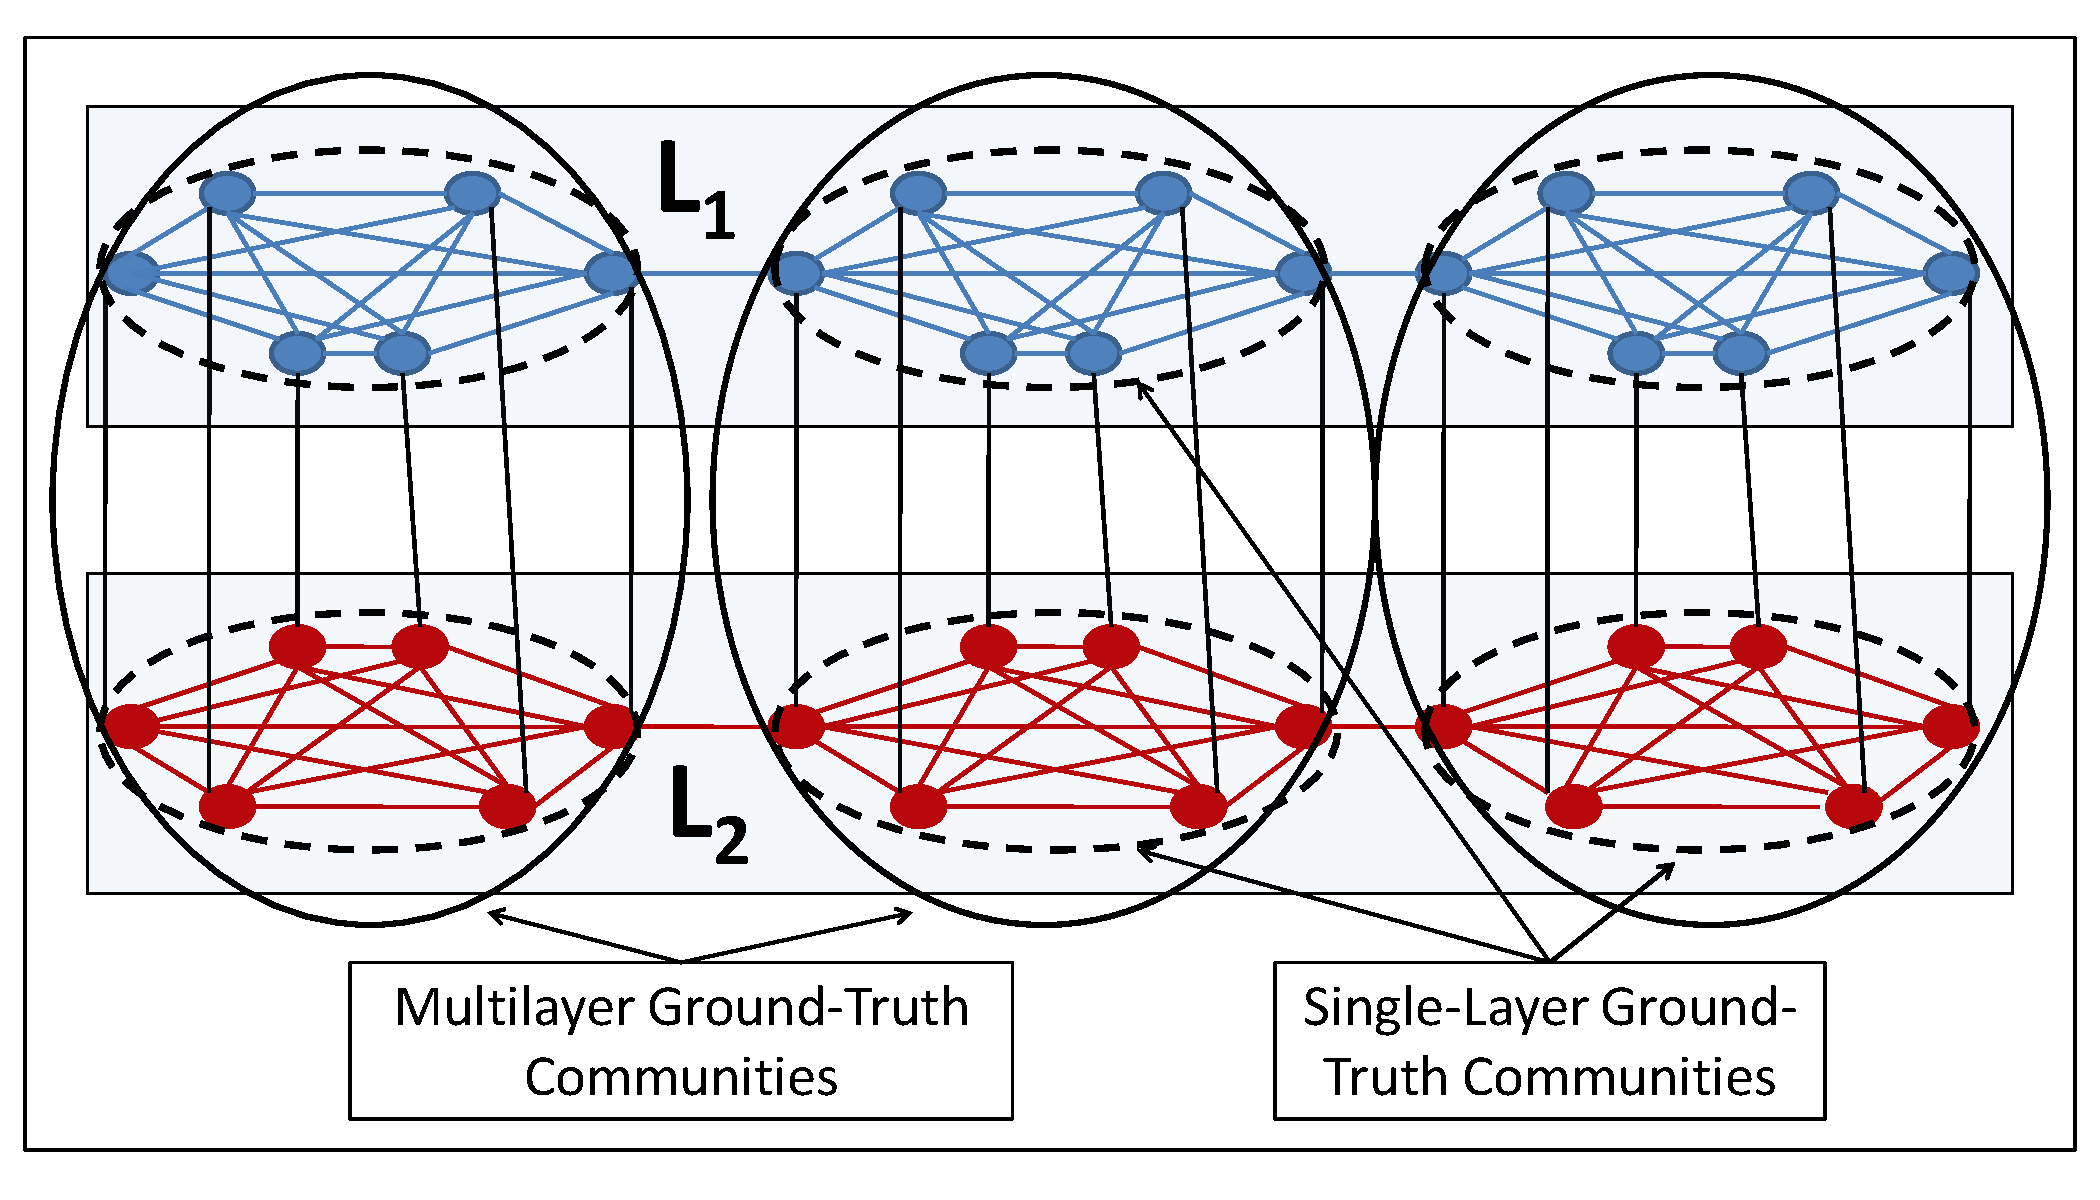
\includegraphics[width=2.5in]{./images/image31.pdf}
% \vspace{-0.1in}
% \caption{Network configuration with two different ground truth communities}
% \label{N0}
% \end{figure}
%
% \begin{figure}
% \centering
% 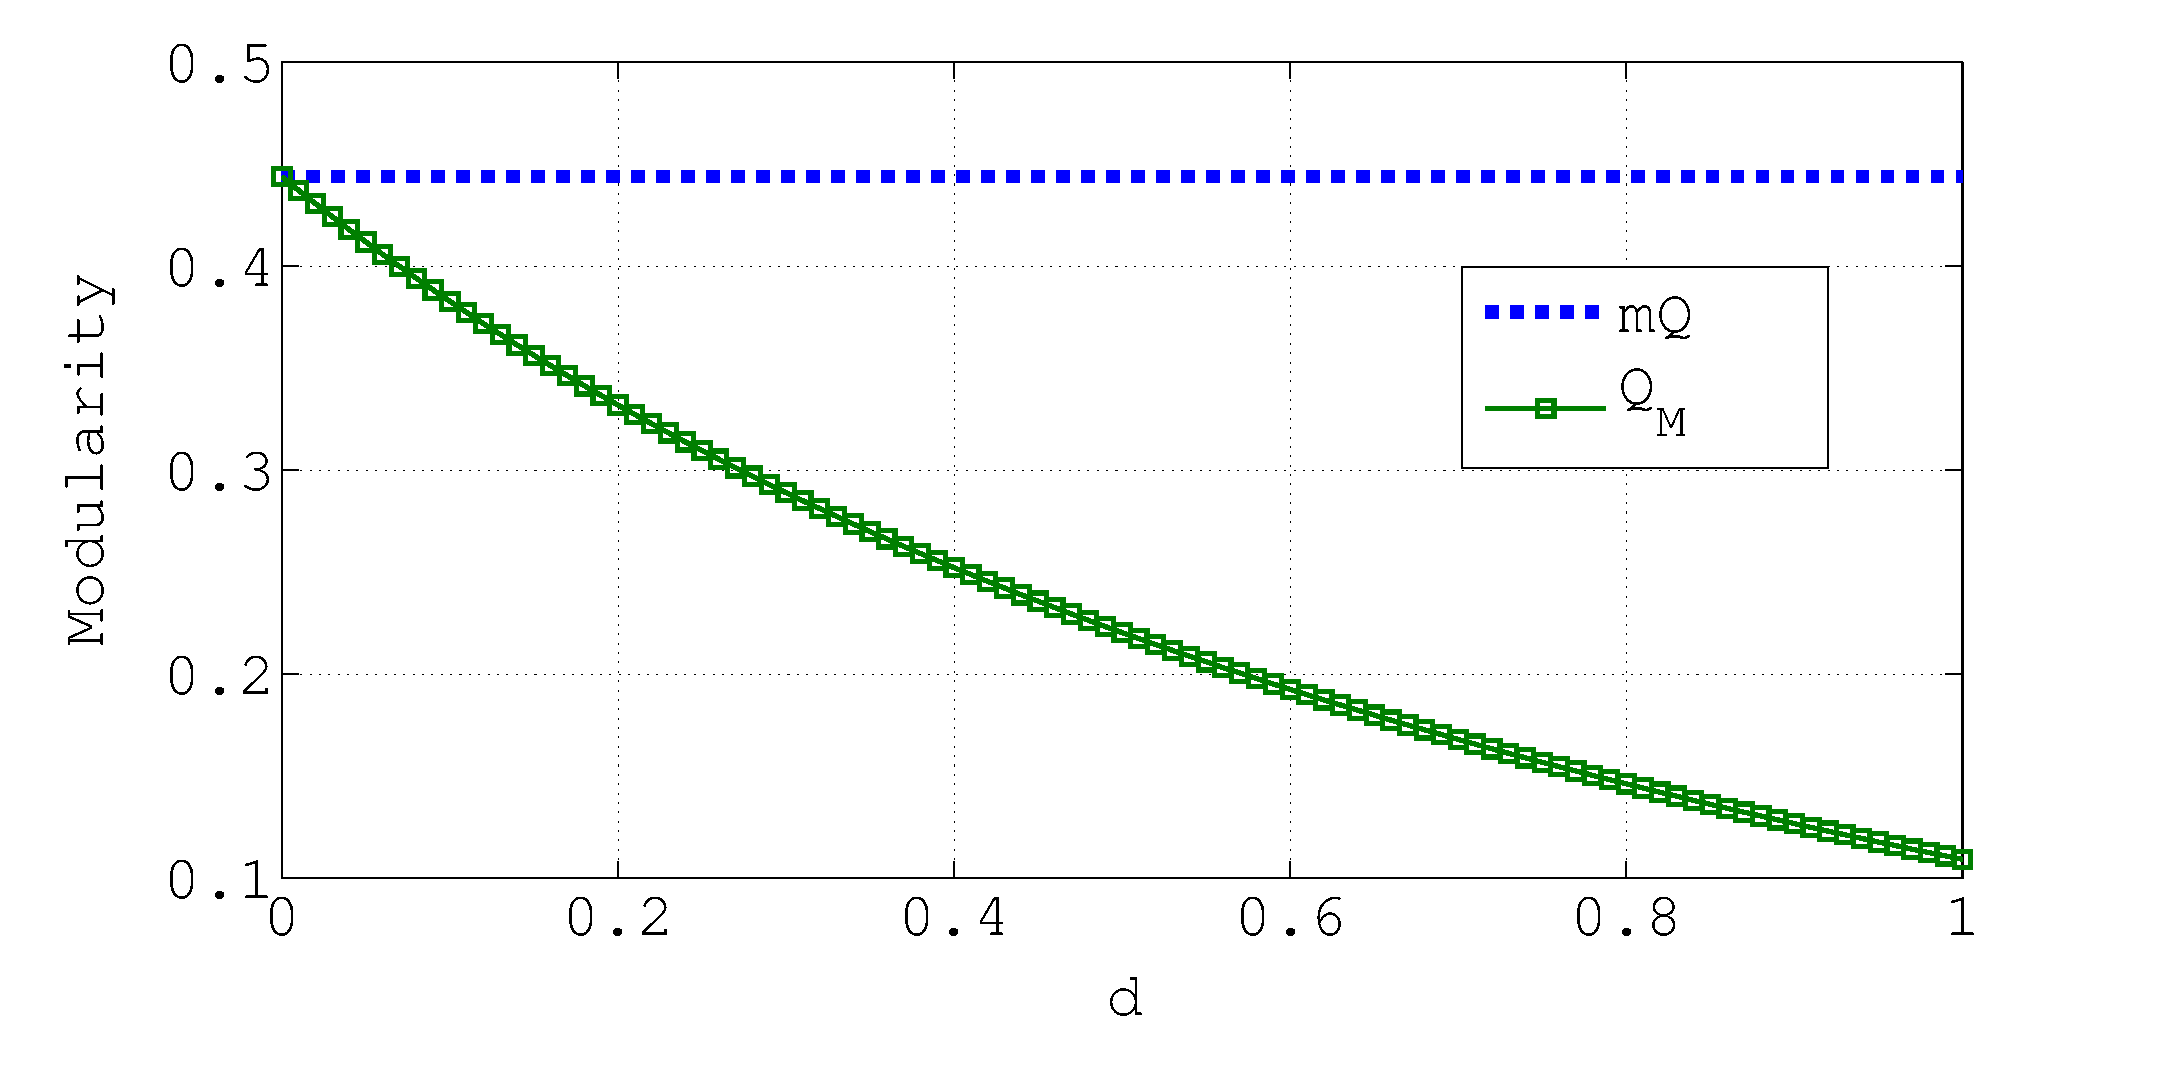
\includegraphics[width=2.5in]{./images/mQ_vs_march21_cross_single.pdf}
% \vspace{-0.1in}
% \caption{Comparison of $mQ$ and $Q_M$ for Config A while adding coupling links with different $P$ values}
% \label{cross_single}
% \end{figure}
%
% \begin{figure}
% \centering
% 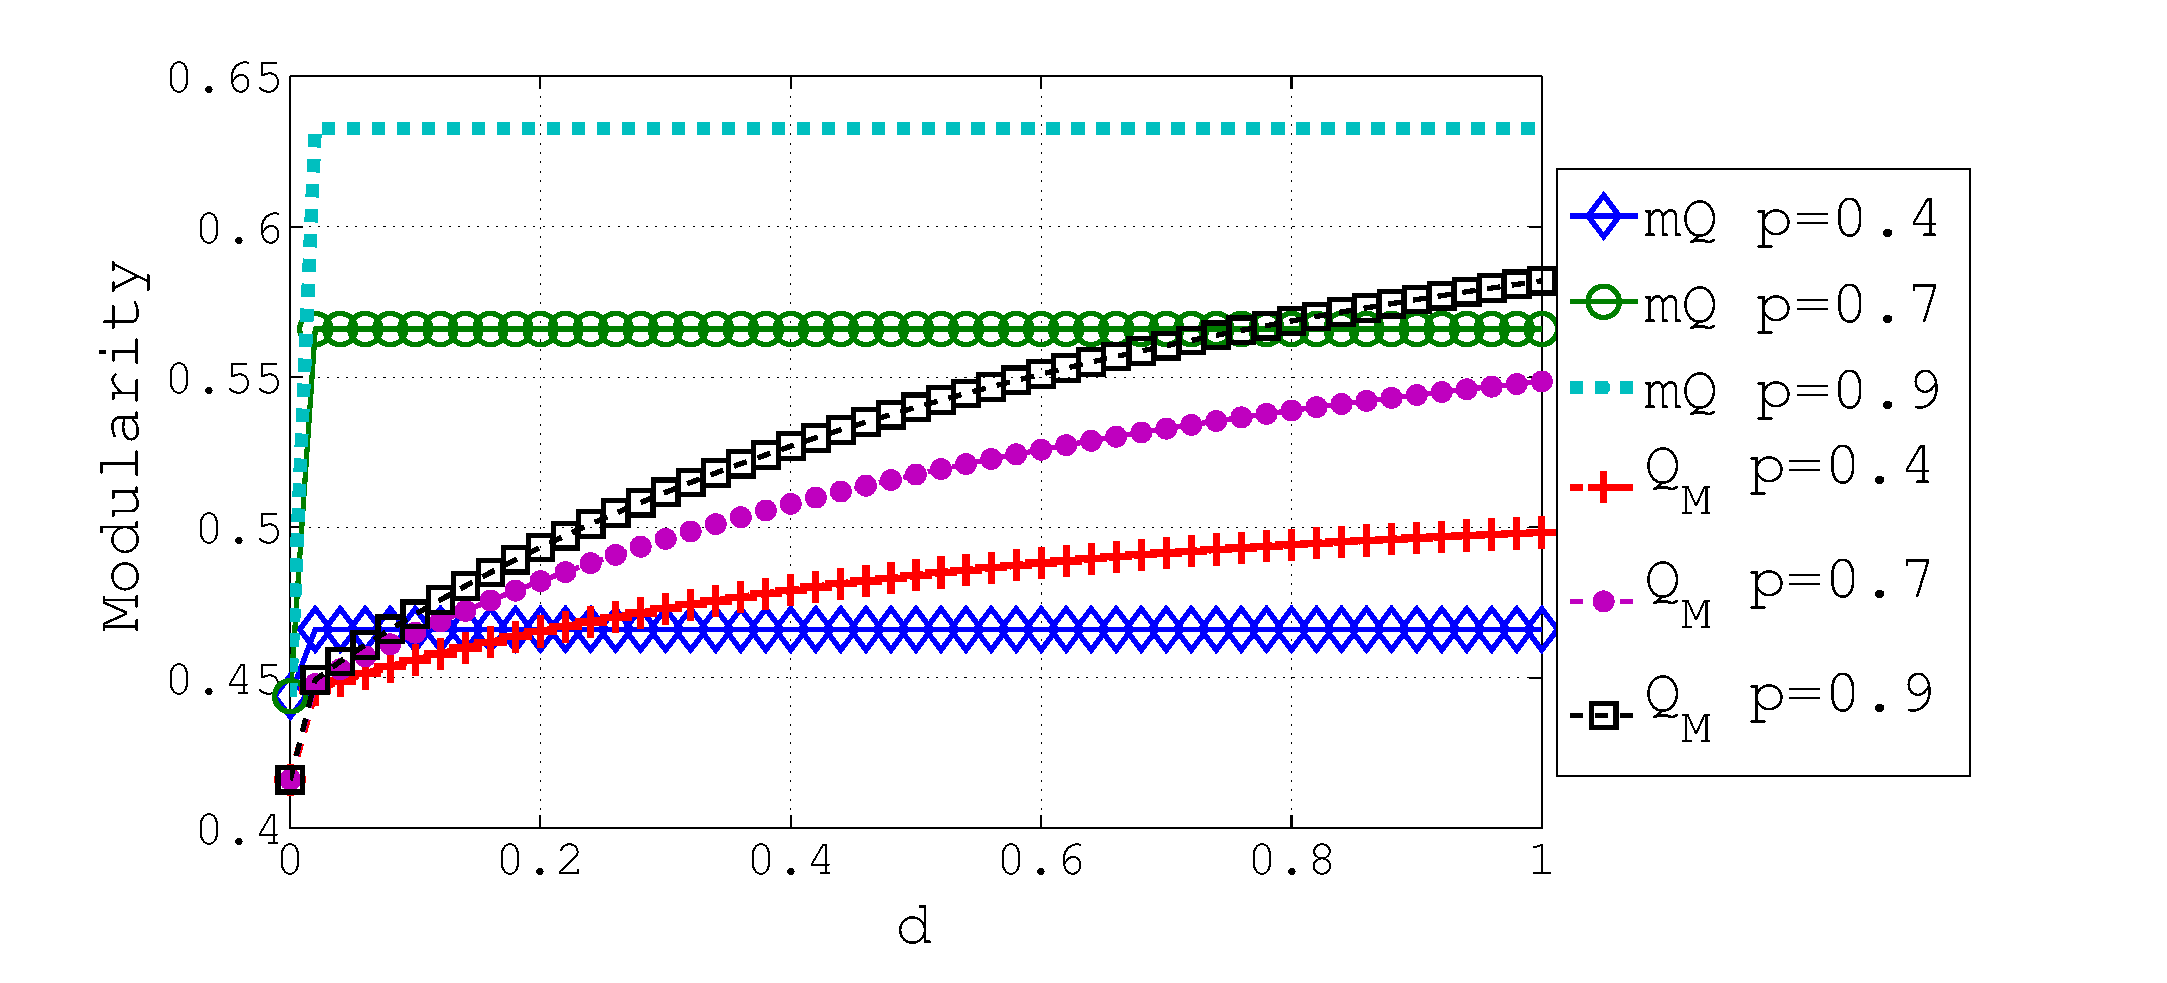
\includegraphics[width=3.5in]{./images/mQ_vs_march21_cross_multi.pdf}
% \vspace{-0.1in}
% \caption{Comparison of $mQ$ and $Q_M$ for Config B while adding coupling links with different $P$ values}
% \label{cross_multi}
% \end{figure}
